\documentclass{beamer}

\definecolor{theme}{HTML}{2471A3}
\definecolor{accent}{HTML}{6272B5}
\definecolor{offblack}{HTML}{2E4053}
\definecolor{pyred}{HTML}{F24532}
\definecolor{pyblue}{HTML}{2E7EBC}
\definecolor{pyorange}{HTML}{FEA862}
\setbeamercolor{normal text}{fg=offblack}

\usecolortheme[named=theme]{structure}
\usecolortheme{rose}
\usecolortheme{dolphin}

% modified version of default frametitle with horizontal separation line
\makeatletter
\setbeamertemplate{frametitle}{
  \ifbeamercolorempty[bg]{frametitle}{}{\nointerlineskip}%
  \@tempdima=\textwidth%
  \advance\@tempdima by\beamer@leftmargin%
  \advance\@tempdima by\beamer@rightmargin%
  \begin{beamercolorbox}[sep=0.3cm,left,wd=\the\@tempdima]{frametitle}
    \usebeamerfont{frametitle}%
    \vbox{}\vskip-2ex%
    \if@tempswa\else\csname beamer@fteleft\endcsname\fi%
    \strut\insertframetitle\strut\par%
    {%
      \ifx\insertframesubtitle\@empty%
      \else%
      {\usebeamerfont{framesubtitle}\usebeamercolor[fg]{framesubtitle}\insertframesubtitle\strut\par}%
      \fi
    }%
    \vskip.45ex%
    \hrule %height .6pt%
    \vskip-1.45ex%
    \if@tempswa\else\vskip-.3cm\fi%
  \end{beamercolorbox}%
}
\makeatother

% clean up footer
\beamertemplatenavigationsymbolsempty
\defbeamertemplate{footline}{custom footline}{
  \usebeamercolor[fg]{page number in head/foot}
  \usebeamerfont{page number in head/foot}
  \quad
  \insertshortauthor\enskip(\insertshortinstitute)
  \hfill
  \insertshorttitle
  \hfill
  \insertframenumber\,/\,\inserttotalframenumber\kern1em\vskip2pt
}
\setbeamertemplate{footline}[custom footline]

\useinnertheme{default}

\setbeamertemplate{itemize items}[circle]
\setbeamercolor{itemize item}{fg=theme!60!white}
\setbeamercolor{itemize subitem}{fg=theme!60!white}

\usepackage{graphicx}
\usepackage[export]{adjustbox}
\graphicspath{{fig/}}

\usepackage[absolute]{textpos}
\usepackage{tcolorbox}

\usepackage{fontawesome}

\usepackage{tikz}
\usepackage{tikzscale}
\usetikzlibrary{calc}
\usetikzlibrary{positioning}
\usetikzlibrary{overlay-beamer-styles}
\usetikzlibrary{arrows}

\usepackage{amsmath}

\usepackage[T1]{fontenc}
%% main font
\usepackage[default]{lato}
%% improves consistency of Greek letters in math mode
%\usepackage{newtxsf}

% alternate font
\usepackage[nosfdefault]{raleway}
% set as the default rm font [even though it really isn't roman]
\renewcommand*\rmdefault{Raleway-TLF}
% and use as the frame title font
\setbeamerfont{frametitle}{family=\rm}

% macros
\newcommand{\trento}{T\raisebox{-0.3ex}{R}ENTo}

\newcommand{\fullwidth}[1]{
  \begin{columns}
    \column{\paperwidth}
    #1
  \end{columns}
}

% tikz grid overlay
\newcommand{\grid}{
  \begin{tikzpicture}[remember picture, overlay]
    \draw[step=1cm, gray, very thin] (current page.south west) grid (current page.north east);
  \end{tikzpicture}
}

% place lead nucleus at tikz coordinate
\newcommand{\lead}[1]{
  \node (position) at (8.8 cm, -5 cm) {\includegraphics[scale=0.27]{#1}};
}

% place lead nucleus at tikz coordinate
\newcommand{\pic}[3]{
  \node (position) at #2 {\includegraphics[scale=#3]{#1}};
}

\newcommand{\tran}{^\intercal}
\newcommand{\T}{\tilde{T}}

\title[Bayesian parameter estimation for HIC]{Bayesian parameter estimation for heavy-ion collisions: inferring properties of the quark-gluon plasma}
\author[J.\ S.\ Moreland]{J.\ S.\ Moreland,\, J.\ E.\ Bernhard,\, W.\ Ke,\, S.\ A.\ Bass}
\institute[Duke U.]{Duke Univerity}
\date{\today}

\begin{document}

\section{Title}


\begin{frame}[t,plain,noframenumbering]
  \centering \vspace{.3\textheight}
  {\color{theme}\large\rm\inserttitle} \\[.04\textheight]
  {\small \insertauthor---Duke U.} \\[1ex]
  {\small XLVII International Symposium on Multiparticle Dynamics\\September 14, 2017}
\end{frame}


\begin{frame}{Lattice predicts existence of a quark-gluon plasma}
  Lattice QCD calculations find a pseudo-critical phase transition temperature $T \approx 155$~MeV, where hadrons melt to form a deconfined soup of quarks and gluons dubbed a quark-gluon plasma (QGP)\\[2ex]
  \begin{columns}
    \begin{column}{0.47\textwidth}
        \includegraphics[width=\columnwidth]{confined_deconfined}
    \end{column}
    \begin{column}{0.4\textwidth}
        \includegraphics[width=\columnwidth]{phasediagram}
    \end{column}
  \end{columns}
\end{frame}

\begin{frame}{What are the quark-gluon plasma bulk properties?}
    \begin{center}
        \begin{tikzpicture}
            \node[anchor=center, yshift=0.75cm] (qgp) at (current page.center) {\includegraphics[width=0.35\textwidth]{qgp}};
            \node[text width=4cm, xshift=3.5cm, yshift=3.5cm] (t1) at (current page.center) {How and under what\\ conditions is it formed\\ in a nuclear collision?};
            \node[text width=4.75cm, xshift=3.5cm, yshift=-1.5cm] (t2) at (current page.center) {How does it recombine\\ to form colorless hadrons?};
            \node[text width=4cm, xshift=-3.5cm, yshift=3cm] (t3) at (current page.center) {Equation of state?\\ Relations between\\ thermal quantities,\\ e.g.\ $P=P(\epsilon)$};
            \node[text width=4cm, xshift=-3.5cm, yshift=-2cm] (t4) at (current page.center) {Transport properties?\\ shear/bulk viscosity,\\ probe energy loss, etc};
            \path[->, >=stealth, theme] ([xshift=-.1cm]t1.west) edge [out=-180, in=90] (qgp.north);
            \path[->, >=stealth, theme] ([yshift=.1cm]t2.north) edge [out=90, in=-30] (qgp.east);
            \path[->, >=stealth, theme] ([xshift=-.8cm]t3.south) edge [out=-90, in=180] (qgp.west);
            \path[->, >=stealth, theme] (t4.east) edge [out=0, in=-90] (qgp.south);
        \end{tikzpicture}
    \end{center}
\end{frame}

\begin{frame}{Formulating an inverse problem}
  \begin{center}
    \only<1>{{\scshape Model-to-data comparison (in an ideal world)} \\[5ex]}
    \only<2>{{\scshape Realistic model-to-data comparison} \\[5ex]}
    \only<3>{{\scshape Parametrize Theory landscape} \\[5ex]}
    \only<4-6>{{\scshape Bayesian parameter estimation} \\[5ex]}
  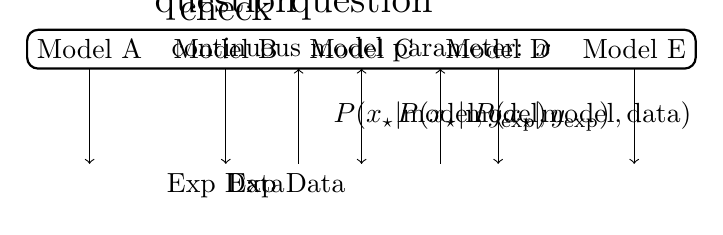
\begin{tikzpicture} 
    \node<1-3>[align=left] (a1) at (current page.center){Model A};
    \node<1-3>[right = 1ex of a1] (b1) {Model B};
    \node<1-3>[right = 1ex of b1] (c1) {Model C};
    \node<1-3>[right = 1ex of c1] (d1) {Model D};
    \node<1-3>[right = 1ex of d1] (e1) {Model E};
    \node<4-6>[align=center] at (c1) {continuous model parameter: $x$};

    \node<1>[above = 0ex of b1, overlay] {\Large \faicon{check}};
    \node<2>[above = 0ex of b1, overlay] {\Large \faicon{question}};
    \node<2>[above = 0ex of c1, overlay] {\Large \faicon{question}};

    \node[below = 8ex of a1] (a2) {};
    \node[below = 8ex of b1] (b2) {};
    \node[below = 8ex of c1] (c2) {};
    \node[below = 8ex of d1] (d2) {};
    \node[below = 8ex of e1] (e2) {};

    \node<1>[below = 8ex of b1] (exp) {Exp Data};
    \node<2-6>[below = 8ex of b1, xshift = 5.1ex] (exp) {Exp Data};

    \draw<1-3>[->] (a1) edge (a2);
    \draw<1-3>[->] (b1) edge (b2);
    \draw<1-3>[->] (c1) edge (c2);
    \draw<1-3>[->] (d1) edge (d2);
    \draw<1-3>[->] (e1) edge (e2);

    \draw<3-6>[thick, rounded corners, overlay] (a1.south west) rectangle (e1.north east);

    \draw<4>[->, transform canvas={xshift=1cm}] (c2) edge (c1);
    \node<4>[below=2ex of c1, transform canvas={xshift=2.8cm}]
    {$P(x_\star| \text{model}, \text{data})$};

    \draw<5>[->, transform canvas={xshift=0cm}] (c2) edge (c1);
    \node<5>[below=2ex of c1, transform canvas={xshift=1.8cm}]
    {$P(x_\star| \text{model}, y_\text{exp})$};

    \draw<6>[->, transform canvas={xshift=-0.8cm}] (c2) edge (c1);
    \node<6>[below=2ex of c1, transform canvas={xshift=1cm}]
    {$P(x_\star| \text{model}, y_\text{exp})$};

    \node<4-6>[below=4ex of c2, overlay, align=center]
    {{\scshape Bayes' Theorem:}\\$\underbrace{P(x_\star| \text{model},\text{data})}_\text{posterior} \propto \underbrace{P(\text{model},\text{data}|x_\star)}_\text{likelihood}\underbrace{P(x_\star)}_\text{prior}$};
  \end{tikzpicture}\\
    \only<7>{
      {\scshape Yields posterior distribution on $x_\star$}\\[2ex]
      \includegraphics[scale=.8]{bayes}\\
      \emph{Includes uncertainty in ``best-fit value''}
    }
  \end{center}
\end{frame}


\begin{frame}{Bayesian parameter estimation in physics}
  \begin{columns}
    \begin{column}{0.4\textwidth}
      \centering {\scshape LIGO Experiment}\\
      \includegraphics[width=\columnwidth]{ligo} \\
      est.\ black hole masses\\
      {\scriptsize PRL 118.221101}\\
    \end{column}
    \begin{column}{0.6\textwidth}
      \begin{itemize}
        \item {\scshape Planck Collaboration 2015:}\\
          constraints on inflation\\
          {\scriptsize Astron.~Astrophys. 594 (2016)}\\[2ex]
        \item CKM parameters\\
          {\scriptsize Eur.~Phys.~J. C21 (2001)}
      \end{itemize}
    \end{column}
  \end{columns}

\end{frame}



\begin{frame}{Quark-gluon plasma is not directly detectable}
    \medskip
    \centering
    \includegraphics[height=0.8\textheight]{qgp_modeling}
\end{frame}


\begin{frame}[plain,t]{Transport models connect experiment and theory}
  \vspace{.075\textheight}
  \begin{enumerate}
    \small
  \item Initial conditions describe $T^{\mu\nu}$ at time $\tau=0^+$
    \item Pre-equilibrium dynamics rapidly drive the system to hydrodynamic applicability
    \item Relativistic viscous hydrodynamics solves $\partial_\mu T^{\mu\nu}=0$,\\
      converts spatial anisotropy into momentum anisotropy
    \item QGP medium is particlized near phase transition temperature
    \item Hadronic afterburner simulates subsequent collisions and decays
  \end{enumerate}
  \includegraphics<1>[width=\textwidth]{hic_picture1}
  \includegraphics<2>[width=\textwidth]{hic_picture3}
  \only<2>{
  \begin{tikzpicture}[remember picture, overlay]
    \node[align=left] (ic) at ([xshift=1.6cm, yshift=-1.9cm]current page.center)
    {\Large\scshape \color{theme} This talk:\\[.5ex]\Large \scshape \color{theme} QGP initial conditions};
    \draw[->, line width=0.4mm, color=theme] (ic.west) -- ([xshift=-1.5cm] ic.west);
  \end{tikzpicture}
  }
\end{frame}


\begin{frame}{Model-to-data comparison: the \emph{inverse} problem}
  \centering \vspace{0.1\textheight}
  \includegraphics[width=\textwidth]{model2data}
\end{frame}

\begin{frame}[plain]
  \begin{columns}
    \begin{column}{.1\textwidth}
    \end{column}
    \begin{column}{.9\textwidth}
    {\Large
    \setbeamercovered{transparent=50}
    \begin{itemize}
      \item<1>[\scshape \color{theme} Part I:] Constructing parametric QGP initial conditions at midrapidity\\[1ex]
      \item<0>[\scshape \color{theme} Part II:] Bayesian parameter estimation\\[1ex]
      \item<0>[\scshape \color{theme} Part III:] Adding nucleon substructure
    \end{itemize}
    }%
    \end{column}
  \end{columns}
\end{frame}

\begin{frame}[t]{QGP initial conditions: sampling nuclei}
  \begin{tikzpicture}[remember picture, overlay]
    \only<1>{\lead{lead_1}}
    \only<2>{\lead{lead_2}}
    \only<3>{\lead{lead_3}}
    \only<4>{\lead{lead_10}}
    \only<5>{\lead{lead_50}}
    \only<6>{\lead{lead_208}}
  \end{tikzpicture}

  {\color{theme} Correlated nucleus algorithm: J.\ Bernhard} \\
  \begin{enumerate}
    \small
    \item Pre-sample nucleon positions from Woods-Saxon dist.\ for nucleus
    \item Place nucleons in order of increasing radii
    \item For each nucleon, sample random $\theta$ and $\phi$ \\
    \item Resample angles if any two nucleons \\
          are too close $|\mathbf{x}_i - \mathbf{x}_j| < d_\mathrm{min}$
  \end{enumerate}

  \begin{columns}
    \begin{column}{.05\textwidth}
    \end{column}
    \begin{column}{.45\textwidth}
      \medskip
      \begin{block}{\centering\small Woods-Saxon Density}
        \medskip
        \centering\small $\displaystyle \rho(r) = \frac{\rho_0}{1 + e^{(r - R_0)/a}}$ \\[2ex]
        \scriptsize Coeff.\ $R_0$ and $a$ for various nuclei from \\
        \textcolor{theme}{Atomic Data and Nuclear Data Tables Vol. 59, Issue 2, 185-381} 
        \smallskip
      \end{block}
    \end{column}
    \begin{column}{.5\textwidth}
    \end{column}
  \end{columns}
\end{frame}

\begin{frame}{Correlated vs uncorrelated nuclei}
  \begin{columns}
    \begin{column}{.5\textwidth}
      \centering
      {\scshape Uncorrelated Pb$^{208}$} \\
      \includegraphics[width=.99\columnwidth]{pb208} \\
      $d_\mathrm{min}=0$~fm
    \end{column}
    \vline
    \begin{column}{.5\textwidth}
      \centering
      {\scshape Correlated Pb$^{208}$} \\
      \includegraphics[width=.99\columnwidth]{pb208_mindist} \\
      $d_\mathrm{min}=1.5$~fm
    \end{column}
  \end{columns}
\end{frame}

\begin{frame}{Collision systems at RHIC and the LHC}
  \centering
  \includegraphics{nuclei}

  \begin{textblock}{1}(3.5, 8.5)
    \centering\scshape U$^{238}$
  \end{textblock}

  \begin{textblock}{1}(7.7, 8.5)
    \centering\scshape Pb$^{208}$
  \end{textblock}
  
  \begin{textblock}{1}(11.9, 8.5)
    \centering\scshape Au$^{197}$
  \end{textblock}

  \begin{textblock}{1}(3.2, 14)
    \centering\scshape Cu$^{62}$
  \end{textblock}

  \begin{textblock}{1}(6.4, 14)
    \centering\scshape He$^{3}$
  \end{textblock}

  \begin{textblock}{1}(9.5, 14)
    \centering\scshape d
  \end{textblock}

  \begin{textblock}{1}(12.5, 14)
    \centering\scshape p
  \end{textblock}

\end{frame}

\begin{frame}[t]{Collision geometry}
  \begin{tikzpicture}[remember picture, overlay]
    \node (a) at (2.3 cm, -3.8 cm) {\includegraphics[scale=0.4]{geometry}};
    \node (a1) at (1 cm, -1.1 cm) {nucleus $A$}; 
    \node (a2) at (3.4 cm, -1.1 cm) {nucleus $B$}; 
    \node (b) at (8.5 cm, -1.5 cm) {\includegraphics[scale=0.3]{traincar-crop}};
    \node (b1) at (8.7 cm, -0.5 cm) {$dS/d\eta \vert_{\eta=0}$}; 
    \node (b2) at (7.7 cm, -2.5 cm) {$T_A$}; 
    \node (b3) at (9.7 cm, -2.5 cm) {$T_B$}; 
    \node (c1) at (8.5 cm, -4.3 cm) {$T(x,y)=\int dz\, \rho_{A,B}(x\pm b,y,z)$}; 
    \node (c2) at (8.5 cm, -5.8 cm) {\large $\dfrac{dS}{d\eta} \Big\vert_{\eta=0} = f(T_A,T_B)$}; 
    \draw [->, line width=0.35mm, color=theme!60!white] (3.1cm, -3.5cm) to[out=10, in=180] (5.4cm, -1.6cm);
  \end{tikzpicture}
\end{frame}

\begin{frame}{Entropy deposition at midrapidity}
  Collisions are stochastic. Entropy deposition mapping only defined on subset of participant matter
  \begin{equation*}
    \frac{dS}{d\eta}\Big\vert_{\eta=0} = f(T_A^\mathrm{part}, T_B^\mathrm{part}),
  \end{equation*}
  where transverse participant density is given by
  \begin{equation*}
    T^\mathrm{part}(x,y) = \sum\limits_{i=1}^{N_\mathrm{part}} T_p(x-x_i, y-y_i),
  \end{equation*}
  and $T_p$ is the proton thickness, typically modeled by a Gaussian.
\end{frame}

\begin{frame}{Entropy deposition scaling with nuclear density?}
  \begin{tikzpicture}[remember picture, overlay]
    \node [yshift=-1.75cm] (t) at (current page.north) {\large Two general approaches:};
    \node [xshift=-3.5cm, yshift=-3cm, align=center] (t) at (current page.north) {Ab initio theory\\calculations};
    \node [xshift=2.5cm, yshift=-3cm, align=center] (t) at (current page.north) {Data-driven\\model inference};
    \node [xshift=-3.5cm, yshift=-4cm, align=center] (t1) at (current page.north) {\small Derive};
    \node [xshift=-2.5cm, yshift=-5cm, align=center] (t2) at (current page.north) {\small Validate};
    \node [xshift=-4.5cm, yshift=-5cm, align=center] (t3) at (current page.north) {\small Refine};
    \node [xshift=-3.5cm, yshift=-6.5cm, align=center] (t4) at (current page.north) {Examples:};
    \node [xshift=-3cm, yshift=-7.5cm, align=left] (t5) at (current page.north) {\small M.V. model\\\small AdS-CFT\\pQCD \& saturation};
    \node [xshift=1cm, yshift=-4cm, align=center] (t6) at (current page.north) {\small Flexible model};
    \node [xshift=2.5cm, yshift=-5.25cm, align=center] (t7) at (current page.north) {\small Bayesian parameter\\estimation};
    \node [xshift=4cm, yshift=-4cm, align=center] (t8) at (current page.north) {\small Experiment};
    \node [xshift=2.5cm, yshift=-6.4cm, align=center] (t9) at (current page.north) {\small Constrained model};
    \node [xshift=2.5cm, yshift=-7.25cm, align=center] (t4) at (current page.north) {Examples in other fields:};
    \node [xshift=2.5cm, yshift=-8cm, align=left] (t10) at (current page.north) {\small LIGO black hole masses\\ \small Cosmological Standard Model};
    \draw [->, line width=0.35mm, color=theme!60!white] (t1.east) to[out=-10, in=90] (t2.north);
    \draw [->, line width=0.35mm, color=theme!60!white] (t2.south) to[out=-90, in=-90] (t3.south);
    \draw [->, line width=0.35mm, color=theme!60!white] (t3.north) to[out=90, in=180] (t1.west);
    \draw [->, line width=0.35mm, color=theme!60!white] (t6.south) to[out=-90, in=120] ([xshift=-1ex]t7.north);
    \draw [->, line width=0.35mm, color=theme!60!white] (t8.south) to[out=-90, in=60] ([xshift=1ex]t7.north);
    \draw [->, line width=0.35mm, color=theme!60!white] (t7.south) -- (t9.north);
  \end{tikzpicture}
\end{frame}

\begin{frame}{\protect\trento\ parametric initial condition model}
    \only<1>{ 
    \begin{tikzpicture}[remember picture,overlay]
        \node[anchor=center, yshift=0.5 cm] at (current page.center) {
            \includegraphics[scale=1]{nucl_offset}};
        \node[below = 1.8cm of current page.center, anchor=north, align=center]{
          Sample nucleon positions from Woods-Saxon density\\with minimum distance criteria $|\mathbf{x}_i - \mathbf{x}_j| > d_\mathrm{min}$};
    \end{tikzpicture}}
   
    \only<2>{ 
    \begin{tikzpicture}[remember picture,overlay]
        \node[anchor=center, yshift=0.5 cm] at (current page.center) {
            \includegraphics[scale=1]{nucl}};
        \node[below = 1.8cm of current page.center, anchor=north, align=center]{
          Nuclei collide at some random impact parameter $b$\\[1ex]
          $dP(b) = 2\pi b\, db$};
    \end{tikzpicture}}
    
    \only<3>{ 
    \begin{tikzpicture}[remember picture,overlay]
        \node[anchor=center, yshift=0.5 cm] at (current page.center) {
            \includegraphics[scale=1]{part}};
        \node[below = 1.8cm of current page.center, anchor=north, align=center]{
          Determine nucleons which participate inelastically\\[1ex]
          $P_\mathrm{coll}(b) = 1 - \exp[-\sigma_{gg} T_{pp}(b)]$,\\[1ex]
          $\sigma_\mathrm{NN}^\mathrm{inel} = \int 2\pi b\, db\, P_\mathrm{coll}(b)$.};
    \end{tikzpicture}}

    \only<4>{ 
    \begin{tikzpicture}[remember picture,overlay]
        \node[anchor=center, yshift=0.5 cm] at (current page.center) {
            \includegraphics[scale=1]{part_offset}};
        \node[below = 1.8cm of current page.center, anchor=north, align=center]{
          Construct participant thickness functions\\[1ex]
          $\displaystyle \T(\mathbf{x}) = \sum\limits_{i=1}^{N_\mathrm{part}} \gamma_i\, \frac{1}{2\pi w^2} \exp\left(-\frac{(\mathbf{x} - \mathbf{x}_i)^2}{2 w^2}\right)$};
    \end{tikzpicture}}

    \only<5>{ 
    \begin{tikzpicture}[remember picture,overlay]
        \node[anchor=center, yshift=0.5 cm] at (current page.center) {
            \includegraphics[scale=1]{thick}};
        \node[below = 1.8cm of current page.center, anchor=north, align=center]{
          Construct participant thickness functions\\[1ex]
          $\displaystyle \T(\mathbf{x}) = \sum\limits_{i=1}^{N_\mathrm{part}} \gamma_i\, \frac{1}{2\pi w^2} \exp\left(-\frac{(\mathbf{x} - \mathbf{x}_i)^2}{2 w^2}\right)$};
    \end{tikzpicture}}
    
    \only<6>{
    \begin{tikzpicture}[remember picture,overlay]
        \node[anchor=center, yshift=0.5 cm] at (current page.center) {
            \includegraphics[scale=1]{entropy}};
          \node[below = 1.8cm of current page.center, align=center, anchor=north] (x2) {
          Convert local overlap density $\rightarrow$ entropy deposition\\[1ex]
          $\displaystyle \frac{dS}{d^2r\, dy}\Big\vert_{y=0} \propto \left(\frac{\T_A^p + \T_B^p}{2}\right)^{1/p}$
        };
        \node[anchor=center, align=left] (x1) at (9.8cm, -3.5cm) {\color{theme} generalized\\\color{theme} mean ansatz};
        \draw[->, color=theme, semithick] (x1.south west) to[out=-120, in=-90] ([xshift=0.85cm]x2.south);
    \end{tikzpicture}}
    
\end{frame}


\begin{frame}{Motivation for the generalized mean ansatz}
    \centering \vspace{.02\textheight}
    \begin{columns}
    \begin{column}{0.9\textwidth}
    \centering
    \begin{tcolorbox}[colback=theme!10, colframe=theme!0]
        \centering \small Generalized mean ansatz: \quad
                   $\displaystyle \frac{dS}{d^2r\, dy} \propto
                    \biggl(\frac{T_A^p + T_B^p}{2}\biggr)^{1/p}$
            \tikz[remember picture] \node[coordinate, above=5 pt] (d1) {};
    \end{tcolorbox}
    \end{column}
    \end{columns}
    \vspace{.06\textheight}
    \begin{columns}[T]
        \begin{column}{0.05\textwidth}
        \end{column}
        \begin{column}{0.7\textwidth}
            \centering
            \includegraphics<1>[width=\textwidth]{thickness_band} 
            \includegraphics<2>[width=\textwidth]{thickness_arithmetic} 
            \includegraphics<3>[width=\textwidth]{thickness_geometric} 
            \includegraphics<4>[width=\textwidth]{thickness_harmonic} 
        \end{column}
        \begin{column}{0.2\textwidth}
            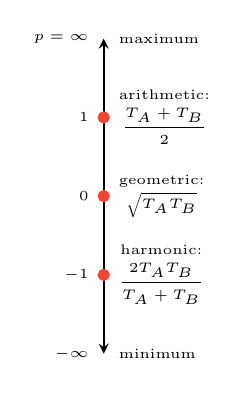
\begin{tikzpicture}
                \tiny
                \tikz[remember picture] \node[coordinate, left=5pt, above=5pt] (d2) {};
                \draw[semithick, <->, >=stealth] (0,0) -- (0,-4);
                \foreach \y in {-1,-2,-3} \draw[semithick] (-2pt, \y cm) -- (2pt, \y cm);
                \draw (0,0) node[left=3pt] {$p=\infty$} node[right=3pt] {maximum};
                \draw (0,-1) node[left=3pt] {$1$} node[right=3pt, align=center] {
                    arithmetic:\\[1ex] $\displaystyle \frac{T_A+T_B}{2}$};
                \draw (0,-2) node[left=3pt] {$0$} node[right=3pt, align=center] {
                    geometric:\\[.4ex] $\displaystyle \sqrt{T_A T_B}$};
                \draw (0,-3) node[left=3pt] {$-1$} node[right=3pt, align=center] {
                    harmonic:\\[1ex] $\displaystyle \frac{2 T_A T_B}{T_A + T_B}$};
                \draw (0,-4) node[left=3pt] {$-\infty$} node[right=3pt] {minimum};
                \draw<2>[pyred, fill=pyred] (0,-1) circle (2 pt);
                \draw<3>[pyred, fill=pyred] (0,-2) circle (2 pt);
                \draw<4>[pyred, fill=pyred] (0,-3) circle (2 pt);
            \end{tikzpicture} 
        \end{column}
        \begin{column}{0.05\textwidth}
        \end{column}
    \end{columns}

    \begin{tikzpicture}[remember picture, overlay]
        \path[->, >=stealth, theme] (d1) edge [out=-45, in=45] (d2);
    \end{tikzpicture}
\end{frame}


\begin{frame}[t]{Parametrization mimics existing theory calculations}
    \medskip
    \only<1-2>{
    \begin{columns}[T]
        \begin{column}{0.3\textwidth}
            \includegraphics[height=0.8\textheight]{cgc_compare}
        \end{column}
        \begin{column}{0.6\textwidth}
            \begin{itemize}
                \itemsep2ex \small
                \item Wounded nucleon model \\[1em]
                      $\displaystyle \frac{dS}{dy\,d^2r_\perp} 
                      \propto T_A + T_B$ \\[1em]
                      {\scriptsize $^*T$ denotes \emph{participant} thickness} 
                \item EKRT model \; {\scriptsize \color{theme} 
                      PRC 93, 024907 (2016)} \\
                      {\scriptsize after brief free streaming phase} \\[1em] 
                      $\displaystyle \frac{dE_T}{dy\,d^2r_\perp}  \sim 
                      \frac{K_\text{sat}}{\pi} p_\text{sat}^3(K_\text{sat}, 
                      \beta; T_A, T_B)$
                \item KLN model \; {\scriptsize \color{theme} PRC 75, 
                     034905 (2007)} \\[1em] $\displaystyle 
                     \frac{dN_g}{dy\,d^2r_\perp} \sim Q^2_{s,\text{min}} \bigg[2 + 
                     \log \bigg(\frac{Q^2_{s,\text{max}}}{Q^2_{s,\text{min}}}
                     \bigg) \bigg]$
            \end{itemize}
        \end{column}
    \end{columns}
  }
  \only<2>{
    \begin{tikzpicture}[remember picture, overlay]
        \filldraw [draw=offblack, fill=offblack, overlay, 
                   opacity=0.3, anchor=center] (current page.south west) 
                   rectangle (\paperwidth,\paperwidth);
        \node[inner sep=0pt, yshift=1cm, overlay] (node1) at 
              (current page.center) {\includegraphics{ipglasma}};
        \node[inner sep=0pt, below=1ex of node1.south, anchor=north] {
            \begin{tcolorbox}[width=0.8\textwidth, boxrule=0pt, 
                              colback=white, colframe=offblack, sharp corners]
                No simple analytic form for IP-Glasma model. However, initial entropy density yield and eccentricity harmonics (above) agree closely with a generalized mean described by $p \approx 0$.
            \end{tcolorbox}
        };
    \end{tikzpicture}
  }

\end{frame}

\begin{frame}{Brief recap}{}
  {\color{theme} \trento\ model:}\\
  \begin{itemize}
    \item Predicts entropy deposition at midrapidity in a relativistic nuclear collision (includes several free parameters).
    \item Parametric construction spans a large subspace of reasonable \emph{ab initio} theory calculations.
  \end{itemize}
  \bigskip
  \textcolor{theme}{Application:}\\
  \begin{itemize}
    \item Answer the \emph{what} without the \emph{why}. How does entropy (energy) deposition scale with nuclear density?
    \item What can we learn about nuclear matter at extreme energy density given the correct initial conditions?
  \end{itemize}

\end{frame}

\begin{frame}{Embed IC in computationally intensive model}
  \bigskip
  Cannot directly observe initial state physics ($\tau \le 3 \cdot 10^{-24}$~s), only final hadrons. Must simulate full spacetime evolution of a relativistic heavy-ion collision. \\[3ex]

  \begin{center}
    \textcolor{theme}{\scshape Hydrodynamic standard model}\\
    {\scriptsize Initial conditions $\rightarrow$ viscous hydrodynamics $\rightarrow$ microscopic hadronic afterburner}\\[1ex]
    \includegraphics[width=\textwidth]{hic_picture1}\\
    {\tiny Fig:\ H.\ Petersen, MADAI collaboration}
  \end{center}

\end{frame}



\begin{frame}[t]{Challenge of rigorous model-to-data comparison}
    \begin{tikzpicture}[overlay, remember picture]
        \node [anchor=east, left=1cm  of current page.north, yshift=-1.8cm] 
            (t1) {\large Parameter};
        \node [anchor=west, right=1cm of current page.north, yshift=-1.8cm] 
            (t2) {\large Observable};
        \node [anchor=east, left=1cm  of current page.north, yshift=-2.4cm] 
            (a1) {\small shear viscosity};
        \node [anchor=east, left=1cm  of current page.north, yshift=-2.9cm] 
            (a2) {\small bulk viscosity};
        \node [anchor=east, left=1cm  of current page.north, yshift=-3.4cm] 
            (a3) {\small pre-equilibrium flow};
        \node [anchor=east, left=1cm  of current page.north, yshift=-3.9cm] 
            (a4) {\small nucleon width};
        \node [anchor=east, left=1cm  of current page.north, yshift=-4.4cm] 
            (a5) {\small hadronization temp};
        \node [anchor=east, left=1cm  of current page.north, yshift=-4.9cm] 
            (a6) {\small p+p fluctuations};
        \node [anchor=west, right=1cm of current page.north, yshift=-2.4cm] 
            (b1) {\small identified yields};
        \node [anchor=west, right=1cm of current page.north, yshift=-2.9cm] 
            (b2) {\small identified mean $p_T$};
        \node [anchor=west, right=1cm of current page.north, yshift=-3.4cm] 
            (b3) {\small flow cumulants};
        \node [anchor=west, right=1cm of current page.north, yshift=-3.9cm] 
            (b4) {\small mode mixing observables};
        \node [anchor=west, right=1cm of current page.north, yshift=-4.4cm] 
            (b5) {\small event plane decorrelations};
        \node [anchor=west, right=1cm of current page.north, yshift=-4.9cm] 
            (b6) {\small HBT interferometry};

        \draw [offblack, line width=0.2pt] (a1.east) -- (b1.west);
        \draw [offblack, line width=0.2pt] (a1.east) -- (b2.west);
        \draw [offblack, line width=0.2pt] (a1.east) -- (b3.west);
        \draw [offblack, line width=0.2pt] (a1.east) -- (b4.west);
        \draw [offblack, line width=0.2pt] (a1.east) -- (b5.west);
        \draw [offblack, line width=0.2pt] (a1.east) -- (b6.west);
        
        \draw [offblack, line width=0.2pt] (a2.east) -- (b1.west);
        \draw [offblack, line width=0.2pt] (a2.east) -- (b2.west);
        \draw [offblack, line width=0.2pt] (a2.east) -- (b3.west);
        \draw [offblack, line width=0.2pt] (a2.east) -- (b4.west);
        \draw [offblack, line width=0.2pt] (a2.east) -- (b5.west);
        \draw [offblack, line width=0.2pt] (a2.east) -- (b6.west);
        
        \draw [offblack, line width=0.2pt] (a3.east) -- (b1.west);
        \draw [offblack, line width=0.2pt] (a3.east) -- (b2.west);
        \draw [offblack, line width=0.2pt] (a3.east) -- (b3.west);
        \draw [offblack, line width=0.2pt] (a3.east) -- (b4.west);
        \draw [offblack, line width=0.2pt] (a3.east) -- (b5.west);
        \draw [offblack, line width=0.2pt] (a3.east) -- (b6.west);

        \draw [offblack, line width=0.2pt] (a4.east) -- (b1.west);
        \draw [offblack, line width=0.2pt] (a4.east) -- (b2.west);
        \draw [offblack, line width=0.2pt] (a4.east) -- (b3.west);
        \draw [offblack, line width=0.2pt] (a4.east) -- (b4.west);
        \draw [offblack, line width=0.2pt] (a4.east) -- (b5.west);
        \draw [offblack, line width=0.2pt] (a4.east) -- (b6.west);

        \draw [offblack, line width=0.2pt] (a5.east) -- (b1.west);
        \draw [offblack, line width=0.2pt] (a5.east) -- (b2.west);
        \draw [offblack, line width=0.2pt] (a5.east) -- (b3.west);
        \draw [offblack, line width=0.2pt] (a5.east) -- (b4.west);
        \draw [offblack, line width=0.2pt] (a5.east) -- (b5.west);
        \draw [offblack, line width=0.2pt] (a5.east) -- (b6.west);
        
        \draw [offblack, line width=0.2pt] (a6.east) -- (b1.west);
        \draw [offblack, line width=0.2pt] (a6.east) -- (b2.west);
        \draw [offblack, line width=0.2pt] (a6.east) -- (b3.west);
        \draw [offblack, line width=0.2pt] (a6.east) -- (b4.west);
        \draw [offblack, line width=0.2pt] (a6.east) -- (b5.west);
        \draw [offblack, line width=0.2pt] (a6.east) -- (b6.west);
    \end{tikzpicture}
    \vspace{.38\textwidth}
    \begin{columns}
    \begin{column}{\textwidth}
    \begin{tcolorbox}[width=\textwidth, colback=theme!10, colframe=theme!0]
      \centering \small \color{offblack}
        Testing a single set of parameters requires $\mathcal{O}(10^4)$ hydro events \\
        \smallskip
        ...and evaluating eight different parameters five times each requires $5^8 \times 10^4 \approx 10^9$ hydro events. \\
        \bigskip
        {\large That's roughly $10^5$ computer \emph{years}!}
    \end{tcolorbox}
    \end{column}
    \end{columns}
\end{frame}


\begin{frame}[plain]
  \begin{columns}
    \begin{column}{.1\textwidth}
    \end{column}
    \begin{column}{.9\textwidth}
    {\Large
    \setbeamercovered{transparent=50}
    \begin{itemize}
      \item<0>[\scshape \color{theme} Part I:] Constructing parametric QGP initial conditions at midrapidity\\[1ex]
      \item<1>[\scshape \color{theme} Part II:] Bayesian parameter estimation\\[1ex]
      \item<0>[\scshape \color{theme} Part III:] Adding nucleon substructure
    \end{itemize}
    }%
    \end{column}
  \end{columns}
\end{frame}


\begin{frame}{Solution: Bayesian parameter estimation}
  \begin{columns}[T]
    \begin{column}{0.25\textwidth}
      \includegraphics[width=.9\columnwidth]{jonah}
    \end{column}
    \begin{column}{.75\textwidth}
      {\scshape \color{theme} Thesis work by Jonah Bernhard} \\[1ex]
      \scriptsize
      \emph{Quantifying properties of hot and dense QCD matter through systematic model-to-data comparison},\\[.5ex]
      Bernhard, et.\ al. PRC 91 (2015). \\[2ex]
      \emph{Applying Bayesian parameter estimation to relativistic heavy-ion collisions: simultaneous characterization of the initial state and quark-gluon plasma medium},\\[.5ex]
      Bernhard, Moreland, Bass, Liu, and Heinz, PRC 94 (2016).
    \end{column}
  \end{columns}
  \bigskip
  \begin{columns}[t]
    \begin{column}{.5\textwidth}
      {\scshape \color{theme} Methodology based on}\\[1ex]
      \scriptsize
      \emph{Computer model calibration using high-dimensional output},\\[.5ex]
      Higdon, Gattiker, Williams, and Rightley,\\ J.Amer.Stat.Assoc.\ 103, 570 (2008).\\[2ex]
      \emph{Determining properties of matter created in ultrarelativistic heavy-ion collisions},\\[.5ex]
      Novak, et. al, PRC 89 (2014).
    \end{column}
    \begin{column}{.5\textwidth}
      {\scshape \color{theme} Used prominently in}\\[1ex]
      \scriptsize
      \emph{Observation of gravitational waves from a binary black hole merger},\\[.5ex]
      LIGO and Virgo collaborations,\\PRL 116 (2016).\\[2ex]
      \emph{Planck 2013 results. Cosmological parameters},\\[.5ex]
      Planck collaboration, Astron.Astrophys.\ 571 (2014).
    \end{column}
  \end{columns}
\end{frame}


\tikzset{
  box/.style={
    align=center,
    inner sep=1ex,
    background default fill=black!10,
    background default text=black!30,
    background fill=theme!15,
    background text=theme,
    fill on=<{1,#1}>,
    text on=<{1,#1}>
  }
}

\newcommand{\boxtitle}[1]{\textbf{#1}\\[.5ex]}

\begin{frame}{Overview: Bayesian parameter estimation}
  \vspace{1em}
  \makebox[\textwidth]{
  \begin{tikzpicture}
    \node[box=1] (input) at (4.5, 6) {
      \boxtitle{Input parameters}
      QGP properties
    };
    \node[box=1] (model) at (8, 4) {
      \boxtitle{Model}
      heavy-ion collision \\
      spacetime evolution
    };
    \node[box=1] (gp) at (1.5, 4) {
      \boxtitle{Gaussian process emulator}
      surrogate model
    };
    \node[box=1] (mcmc) at (3.5, 2) {
      \boxtitle{MCMC}
      calibrate model to data
    };
    \node[box=1] (posterior) at (8, .5) {
      \boxtitle{Posterior distribution}
      quantitative estimates \\
      of each parameter
    };
    \node[box=1] (exp) at (.5, .3) {
      \boxtitle{Experimental data}
      LHC Pb-Pb collisions
    };
    \begin{scope}[color=black!70, ->, semithick]
      \draw (input) -| (model);
      \draw (model) -- (gp);
      \draw (input) -| (gp);
      \draw
        let \p1 = (gp.south), \p2 = (mcmc.north), \p3 = ($(\p1)!.5!(\p2)$) in
        (\p1) -- (\x1, \y3)  -| (\p2);
      \draw (exp) |- (mcmc);
      \draw (mcmc) -| (posterior);
    \end{scope}
  \end{tikzpicture}
}
\end{frame}


\begin{frame}{Details: heavy-ion collision model}
  \smallskip
  \begin{columns}[T]
      \begin{column}{.075\textwidth}
      \end{column}
      \begin{column}{.2\textwidth}
        \centering \medskip
        \includegraphics[height=.75\textheight]{evolution} \\[1ex]
        \tiny Fig: Zhi Qiu
      \end{column}
      \begin{column}{.7\textwidth}
        \begin{itemize}
          \item \textcolor{theme}{\trento\ initial conditions} \\[.5ex]
            {\scriptsize \emph{Parametric entropy deposition}\\
            Moreland, Bernhard, Bass, PRC 92, 011901 (2015)}
          \item \textcolor{theme}{Pre-equilibrium freestreaming} \\[.5ex]
            {\scriptsize \emph{Initial (infinitely) weak coupling phase} \\
            Liu, Chen, Heinz, PRC 91, 064906 (2015)} 
          \item \textcolor{theme}{HotQCD equation of state} \\[.5ex]
            {\scriptsize \emph{Lattice QCD (2+1)-flavor EoS} \\
            Bazavov, et.\ al.\ PRD 90, 094503 (2014)} \\
          \item \textcolor{theme}{iEBE-VISHNU hydrodynamics} \\[.5ex]
            {\scriptsize \emph{Boost-invariant shear+bulk viscous hydrodynamics}\\
            Shen, et. al, Comp.\ Phys.\ Comm.\ 199, 61 (2016)}  
          \item \textcolor{theme}{UrQMD hadronic afterburner} \\[.5ex]
            {\scriptsize \emph{Simulates hadronic rescattering and resonance decay} \\
            Bass et.\ al, Prog.\ Part.\ Nucl.\ Phys.\ 41, 255 (1998)}
        \end{itemize}
      \end{column}
      \begin{column}{.025\textwidth}
      \end{column}
    \end{columns}

  \begin{tikzpicture}[remember picture, overlay]
    \draw[->, semithick, color=theme] (.5cm,7.4cm) -- (.5cm,0.9cm);
    \node[rotate=90, color=theme] at (.25cm, 4.2cm) {time};
  \end{tikzpicture}
\end{frame}


\begin{frame}{Experimental calibration data}
    \begin{center}
    All experimental data from the ALICE collaboration at the LHC \\
    Pb-Pb collisions at $\sqrt s = 2.76$ and 5.02 TeV
  \end{center}
  \begin{columns}
    \column{.6\textwidth}
    Centrality dependence of: \\[1ex]
    \begin{itemize}
      \setlength{\itemsep}{1.5ex}
      \item Charged particle yields $dN_\text{ch}/d\eta$ \\
        {\tiny PRL 106 032301 [1012.1657], PRL 116 222302 [1512.06104]}
      \item Identified particle ($\pi$, $K$, $p$) yields $dN/dy$
        and mean transverse momenta $\langle p_T \rangle$ (2.76 TeV only) \\
        {\tiny PRC 88 044910 [1303.0737]}
      \item Anisotropic flow cumulants $v_n\{2\}$ \\
        {\tiny PRL 116 132302 [1602.01119]}
    \end{itemize}
    \column{.4\textwidth}
    \centering
    \includegraphics[height=.25\textheight]{nch}
    \hfill
    \includegraphics[height=.25\textheight]{spectra} \\
    \includegraphics[height=.4\textheight]{flow}
  \end{columns}
\end{frame}

\begin{frame}{Model input parameters}
  \definecolor{emph}{rgb}{.91,.41,.17}
  \begin{columns}
    \column{.55\textwidth}
    Initial condition
    \begin{itemize}
      \item \trento\ entropy deposition $p$
      \item Multiplicity fluctuation $\sigma_\text{fluct}$
      \item Gaussian nucleon width $w$
    \end{itemize}
    \medskip
    Pre-equilibrium
    \begin{itemize}
      \item Free streaming time $\tau_\text{fs}$
    \end{itemize}
    \medskip
    QGP medium
    \begin{itemize}
      \item $\eta/s$ min, slope, curvature
      \item $\zeta/s$ max, width
      \item $T_\text{switch}$ (hydro to UrQMD)
    \end{itemize}
    \column{.5\textwidth}
    \begin{center}
      \textbf{Latin hypercube design}
    \end{center}
    500 semi-random, space-filling parameter points;
    ${\sim}3 \times 10^4$ min-bias events per point \\[1em]
    \includegraphics{design}
  \end{columns}
\end{frame}


\begin{frame}{Evaluating the model at each design point}
  \begin{tikzpicture}[remember picture, overlay]
    \node at ([yshift=-1ex]current page.center) {\includegraphics[width=.95\paperwidth]{observables_design}};
  \end{tikzpicture}
\end{frame}

\begin{frame}{Training the emulator}
  \vspace{1em}
  \begin{columns}[c]
    \column{.58\textwidth}
    Gaussian process:
    \begin{itemize}
      \item Stochastic function: maps inputs to normally-distributed outputs
      \item Specified by mean and covariance functions
    \end{itemize}
    \bigskip
    As a model emulator:
    \begin{itemize}
      \item Non-parametric interpolation
      \item Predicts \emph{probability distributions}
        \begin{itemize}
          \item Narrow near training points, \\ wide in gaps
        \end{itemize}
      \item Fast surrogate to actual model
    \end{itemize}
    \column{.45\textwidth}
    \includegraphics{gp}
  \end{columns}
\end{frame}


\newcommand{\ydiff}{(\mathbf y - \mathbf y_\text{exp})}
%
\begin{frame}{Markov-chain Monte Carlo}
  \medskip
    Perform random walk through parameter space, weighted by the Bayesian posterior probability:
  \begin{center}
    \textbf{Bayes' theorem} \\
    posterior ${}\propto{}$ likelihood ${}\times{}$ prior
  \end{center}
  Prior = flat in design space \\[1ex]
  Likelihood${} \propto \exp\bigl[ -\frac{1}{2} \ydiff\tran \Sigma^{-1} \ydiff \bigr]$ \\[.5ex]
  \begin{itemize}
    \setlength{\itemsep}{.8ex}
    \item $\Sigma = \text{covariance matrix} = \Sigma_\text{experiment} + \Sigma_\text{model}$
    \item $\Sigma_\text{experiment} = {}$stat (diagonal) + sys (non-diagonal)
    \item $\Sigma_\text{model}$ conservatively estimated as 5\% (to be improved)
  \end{itemize}
  \smallskip
  \begin{tcolorbox}[width=\textwidth, colback=theme!10, colframe=theme!0]
    \emph{\color{theme} Posterior dist.\ determined from equilibriated walker density}
  \end{tcolorbox}
\end{frame}


\begin{frame}[b]{Model calibration}
  \begin{tikzpicture}[remember picture, overlay]
    \only<1>{
      \node at (current page.center) {
        \includegraphics[width=.95\paperwidth]{observables_design}
      };
    }
    \only<2>{
      \node at (current page.center) {
        \includegraphics[width=.95\paperwidth]{observables_posterior}
      };
    }
  \end{tikzpicture}
  \begin{center}
    \only<1>{\color{theme} Model calculations at each of the 500 design points}
    \only<2>{\color{theme} One-hundred random samples drawn from the posterior}
  \end{center}
\end{frame}


\begin{frame}[label=posterior, plain]
  \includegraphics[height=\paperheight]{posterior}
  \begin{tikzpicture}[remember picture, overlay]
    \only<1>{
      \node[below left=1em and 2.5em of current page.north east, color=theme, font=\Large\rm]
      (title) {
        Posterior distribution
      };
      \node[below=1ex of title, anchor=north, font=\small, align=left] {
          Diagonals: prob.\ dists.\ of each param. \\
          Off-diagonals: correlations b/w pairs \\[1ex]
          Estimated values: medians \\
          Uncertainties: 90\% credible intervals%
      };
    }
    \only<2>{
      \node[below left=2em and 1em of current page.north east] (x1) {
          \includegraphics[width=0.5\textwidth]{posterior_p}
      };
      \draw [->, semithick, color=theme] ([xshift=0.2cm, yshift=0.5cm]x1.south west) to[out=-120, in=60] (-8.1cm,9cm); 
      \node [xshift=3.5cm, yshift=0.5cm, align=center] at (current page.center) {Entropy deposition scales\\with geometric mean\\of nuclear density\\[1ex] $dS/dy \approx \sqrt{\rho_A \,\rho_B}$};
    }
  \end{tikzpicture}
\end{frame}

\begin{frame}{Geometric mean scaling in the literature}
  \begin{tcolorbox}[title=AdS-CFT holography, colframe=theme!60!white, colback=theme!02]
  {\small \textcolor{theme}{\emph{Pre-equillibrium radial flow from central shock-wave collisions in AdS5}, Paul Romatschke, J.\ Drew Hogg, JHEP 1304 (2013) 048.}\\[1ex]
    ``We find that the early-time radial flow buildup is identical to that expected from ideal hydrodynamics with an entropy density proportional to the square root of the product of the matter densities in the individual nuclei.''}
  \end{tcolorbox}
  \smallskip
  \begin{tcolorbox}[title=Color flux-tube model, colframe=theme!60!white, colback=theme!02]
    {\small Collision process with $\nu$ soft gluon exchanges akin to random-walk in color space. Strength of effective color charge $Q \propto \sqrt{\nu}$. Particle production (entropy) scales like\, $dN/dy \propto \sqrt{\rho_A\, \rho_B}$}.
  \end{tcolorbox}
\end{frame}


\begin{frame}[plain,t]
  \fullwidth{
    \centering
    \includegraphics<1>[width=.95\paperwidth]{observables_map.png}
    \includegraphics<2>[width=.95\paperwidth]{observables_map.pdf}
  }
  \bigskip
  \scriptsize
  \setbeamercolor{lightbg}{bg=theme!10!white}
  \only<2>{
  \begin{beamercolorbox}[sep=1ex]{lightbg}
    \trento\ $p = 0$
    \hfill
    $\sigma_\text{fluct} = 1$
    \hfill
    $w = 0.9$ fm
    \hfill
    $\tau_\text{fs} = 0.6$ fm/$c$
    \hfill
    $T_\text{switch} = 150$ MeV
    \\[1ex]
    $\eta/s$ min = 0.06, \enskip slope = 2.2 GeV$^{-1}$, \enskip crv = $-0.4$
    \hfill
    $\zeta/s$ max = 0.015, \enskip width = 0.01 GeV
  \end{beamercolorbox}
  }
  \only<1>{
    \begin{tikzpicture}[remember picture, overlay]
      \node at ([yshift=2em]current page.center) {
        \begin{tcolorbox}[colback=theme!20!offblack, colframe=theme, boxrule=0pt, opacityframe=.8, opacityback=.8]
          \centering
          \LARGE\color{white} What's the best the model can do?
        \end{tcolorbox}
      };
    \end{tikzpicture}
  }
\end{frame}


\begin{frame}{Checking non-calibrated flow observables}
  Correlations between event-by-event fluctuations of the magnitudes of flow harmonics m and n:
  \begin{equation*}
    \text{SC}(m, n) = \langle v_m^2 v_n^2 \rangle - \langle v_m^2 \rangle \langle v_n^2 \rangle 
  \end{equation*}
    \includegraphics{flow_corr} \\[1ex]
    \hfill \tiny Data: ALICE, PRL 117 182301 [1604.07663]
\end{frame}


\begin{frame}[plain]{Success of saturation models + hydro}
  \centering
  \medskip
  \scriptsize Hydro models with saturation IC, e.g.\ \trento, IP-Glasma and EKRT,\\
  provide excellent description of bulk observables in A+A collisions \\[1ex]
  \includegraphics[width=.8\textwidth]{mode_observables} \\[1ex]
  \begin{textblock*}{0.3\textwidth}(9.5 cm, 2.0 cm)
    \rotatebox{-90}{\tiny PRC 94, 024907 [1605.03954]}
  \end{textblock*}
  \begin{columns}
    \begin{column}{.075\textwidth}
    \end{column}
    \begin{column}{.45\textwidth}
      \centering
      \includegraphics[width=\columnwidth]{vn_ipglasma.eps} \\
      {\tiny PRL 113, 102301 [1405.3605]}
    \end{column}
    \begin{column}{.4\textwidth}
      \centering
      \includegraphics[width=.91\columnwidth]{vn_ekrt} \\
      {\tiny PRC 93, 024907 [1505.02677]}
    \end{column}
    \begin{column}{.075\textwidth}
    \end{column}
  \end{columns}
\end{frame}


\begin{frame}{Aside: agreement validates scaling, not narrative!}
  \begin{itemize}
  \large
  \item[\faicon{question-circle-o}] How do we proceed if two models with different narratives predict similar initial conditions?\\[2ex] 
  \item[\faicon{wrench}] How can we disambiguate model scaling behavior and the underlying theoretical framework?
  \end{itemize}
  \begin{center}
    These questions aside: there is strong evidence that saturation-\emph{like} effects govern particle production in relativistic nuclear collisions and their magnitude is well constrained.\\[2ex]
    This work:\quad $\dfrac{dS}{d^2r\,dy}\Big\vert_{y=0} \approx \sqrt{\rho_A \,\rho_B}$\\[2ex]
    \emph{Purely observational inference! Need not be exact,\\but robust to moderate perturbations.}
  \end{center}
\end{frame}


\begin{frame}[plain]
  \begin{columns}
    \begin{column}{.1\textwidth}
    \end{column}
    \begin{column}{.9\textwidth}
    {\Large
    \setbeamercovered{transparent=50}
    \begin{itemize}
      \item<0>[\scshape \color{theme} Part I:] Constructing parametric QGP initial conditions at midrapidity\\[1ex]
      \item<0>[\scshape \color{theme} Part II:] Bayesian parameter estimation\\[1ex]
      \item<1>[\scshape \color{theme} Part III:] Adding nucleon substructure
    \end{itemize}
    }%
    \end{column}
  \end{columns}
\end{frame}

\begin{frame}{Flow-like signatures observed in small systems}
  \medskip
  Naively, hydrodynamic behavior was only expected in heavy-ion collisions, \emph{not} in 
  proton-proton and proton-lead collisions.
  \begin{center}
    \Large \color{theme}
    ``When does hydrodynamics turn on/off?''
  \end{center}
  \medskip
  \includegraphics[width=.5\textwidth]{corr2D_PbPb}
  \includegraphics[width=.5\textwidth]{corr2D_pPb}
  \begin{tikzpicture}[remember picture, overlay]
    \node (f1) at ([xshift=-1.2cm, yshift=-1.6cm]current page.center) {};
    \node (f2) at ([xshift=3cm, yshift=-2.25cm]current page.center) {};
    \node (txt) [align=center] at ([yshift=-4cm]current page.center) {\scshape \color{pyred} Long-range rapidity correlations\\\color{pyred}\scshape characteristic of flow};
    \draw [->, thick, color=pyred] (txt.north) to[out=90, in=0] (f1);
    \draw [->, thick, color=pyred] (txt.north) to[out=90, in=120] (f2);
  \end{tikzpicture}
\end{frame}

\begin{frame}{What if we apply A+A models to small systems?}
  \centering
  {\tiny PHENIX submitted to PRC [1609.02894]} \\
  \includegraphics[width=.85\columnwidth]{phenix_models} \\[1ex]
  \small IP-Glasma + hydro model could not reproduce experimental\\multiparticle correlations in small systems... what's wrong? \\[1ex]
  \setbeamercovered{transparent=50}
  \begin{itemize}
    \item<1> Perhaps hydro isn't valid, incorporate initial CGC correlations
    \item<1-2> Saturation IC + hydro correct picture, small systems require additional nucleon substructure
  \end{itemize}
  \scriptsize Note: SONIC model pictured above has not demonstrated same level\\
  of agreement as IP-Glasma + hydro in Pb+Pb collisions
\end{frame}


\begin{frame}{"Eccentric protons?" \quad {\scriptsize \textcolor{offblack}{Schenke, Venugopalan PRL 113 102301}}}
  \small
  \begin{itemize}
    \item Data highly constrains functional form of entropy deposition.\\[1ex]
    \item Cannot modify mapping without spoiling bulk A+A observables, but \emph{we can} add
          fine structure to the inputs (thickness functions)\\[2ex]
  \end{itemize}
  \centering
  \only<1>{\includegraphics[width=.8\textwidth]{Pb_thick}}
  \only<2>{\includegraphics[width=.8\textwidth]{p_thick}} \\[2ex]
  \only<1>{Historical analogue: nucleon hot spots necessary for triangular flow}
  \only<2>{Possibly similar picture for partons inside the nucleon?}

\end{frame}

\begin{frame}{Theory perspective: proton shape fluctuations}
  \medskip
  \begin{columns}
    \begin{column}{.6\textwidth}
      {\color{theme} \scshape Several important contributions:} \\[1ex]
      {\small
      \emph{Shapes of the proton},\\Gerald A.\ Miller, PRC 68 (2003) 022201 \\[1ex]
      {\color{theme} Spin-dependent proton shape fluctuations}\\
      \medskip\hrule\medskip
      \emph{Revealing proton shape fluctuations with incoherent diffraction at high energy},\\ M\"antysaari, Schenke, PRD 94, 034042 \\[1ex]
      \emph{Evidence of strong proton shape fluctuations from incoherent diffraction},\\ M\"antysaari, Schenke, PRL 117, 052301 \\[1ex]
      {\color{theme} Work to implement proton shape fluctuations within IP-Glasma. Shape parameters constrained by J/$\Psi$ differential cross section.}
      }%
    \end{column}
    \begin{column}{.4\textwidth}
      \centering
      \includegraphics[width=.9\columnwidth]{density_lumpy}\\
      \includegraphics[width=.9\columnwidth]{density_smooth}\\
      {\tiny Various lumpy proton shapes input to IP-Sat}
    \end{column}
  \end{columns}

\end{frame}

\begin{frame}
  \begin{columns}
    \begin{column}{.9\textwidth}
    \centering
    {\Large \color{theme} \rm This work:}\\
    \begin{itemize}
      \large
      \item Implement parametric nucleon substructure within the \trento\ initial condition model
      \item Estimate new substructure parameters using Bayesian methodology 
    \end{itemize}
    \end{column}
  \end{columns}
\end{frame}


\begin{frame}[t]{\trento\ model with nucleon substructure}
  \vspace{.1\textheight}
  \begin{columns}[t]
    \begin{column}{.5\textwidth}
      \centering
      {\color{theme} \scshape \Large Nucleon dof} \\[1ex]
      \includegraphics<1>{pp_part}
      \includegraphics<2>{pp_thick}
      \includegraphics<3>{pp_overlap}
      \includegraphics<4>{pp_entropy}\\
    \end{column}
    \begin{column}{.5\textwidth}
      \centering
      {\color{theme} \scshape \Large Parton dof} \\[1ex]
      \includegraphics<1>{pp_part_partons}
      \includegraphics<2>{pp_thick_partons}
      \includegraphics<3>{pp_overlap_partons}
      \includegraphics<4>{pp_entropy_partons}\\
    \end{column}
  \end{columns}
  \medskip
  \only<1>{
    \smallskip
    \begin{columns}[t]
      \begin{column}{.02\textwidth}
      \end{column}
      \begin{column}{.48\textwidth}
        \begin{itemize}
          \item Nucleon width [fm]
        \end{itemize}
      \end{column}
      \begin{column}{.02\textwidth}
      \end{column}
      \begin{column}{.48\textwidth}
        \begin{itemize}
          \item Nucleon width [fm]
          \item Parton width [fm]
          \item Parton number
        \end{itemize}
      \end{column}
    \end{columns}
  }
  \only<2>{
    \begin{columns}[t]
      \begin{column}{.45\textwidth}
        \centering Gaussian nucleons\\[2ex]
        \small $\displaystyle T_p(\mathbf{x}) = \frac{1}{2\pi w^2} \exp\Big({-}\frac{\mathbf{x}^2}{2 w^2}\Big)$
      \end{column}
      \begin{column}{.55\textwidth}
        \centering Sum of Gaussian partons
        {\small
        \begin{align*}
          T_p(\mathbf{x}) &= \sum\limits_{i=1}^{N_\mathrm{partons}} \frac{1}{2\pi v^2} \exp\Bigr({-}\frac{|\mathbf{x} - \mathbf{x}_i|^2}{2 v^2}\Bigr) \\
          P(|\mathbf{x}_i|) &\sim \exp[-0.5\, r^2/(w^2-v^2)]
        \end{align*}
        }%
      \end{column}
    \end{columns}
  }
  \only<3>{
    \centering Sample proton-proton inelastic cross section
    \begin{align*}
      T_{pp}(b) &= \int d^2x\, T_p(\mathbf{x} + \mathbf{b})\, T_p(\mathbf{x}) \\
      P_\mathrm{coll}(b) &= 1 - \exp[-\sigma_{gg} T_{pp}(b)]\\
      \sigma_\mathrm{NN}^\mathrm{inel} &= \int 2\pi b\, db\, P_\mathrm{coll}(b)
    \end{align*}
  }
  \only<4>{
    \centering Entropy density scales with generalized mean\\ of participant nucleon density, e.g. \\[2ex]
    $\displaystyle \frac{dS}{d^2r\, dy}\Big\vert_{y=0} \propto \sqrt{T_A T_B}$
    \begin{tikzpicture}[remember picture, overlay]
      \node (mean) [align=left] at (1.5, 0) {\color{theme} geometric\\ \color{theme} mean};
      \draw [->, color=theme, semithick] (mean.south west) to[out=-120, in=-90] (-.5, -.3);
    \end{tikzpicture}
  }

\end{frame}


\begin{frame}{Substructure effect on nuclear thickness functions}
  \smallskip
  \begin{columns}
    \begin{column}{.02\textwidth}
      \rotatebox{90}{\small Parton width [fm]}
    \end{column}
    \begin{column}{.49\textwidth}
      \centering Lead nucleus \\ 
      \includegraphics[height=\columnwidth]{Pb_thickness} \\
      \small Parton number
    \end{column}
    \begin{column}{.49\textwidth}
      \centering Proton \\
      \includegraphics[height=\columnwidth]{p_thickness} \\
      \small Parton number
    \end{column}
  \end{columns}
  \vspace{.75 cm}
  \centering
  \small nucleon width fixed, $w = 0.5$~fm
\end{frame}


\begin{frame}{Substructure effect on initial entropy density}
  \centering
  \only<1>{
    {\color{theme} \rm \trento: Pb+Pb, $\sqrt{s_\mathrm{NN}}=2.76$~TeV, $p=0$, $w=0.88$~fm} \\[1ex]
  }
  \only<2>{
    {\color{theme} \rm \trento: p+Pb, $\sqrt{s_\mathrm{NN}}=2.76$~TeV, $p=0$, $w=0.88$~fm} \\[1ex]
  }
  \includegraphics<1>[width=\textwidth]{ic_prop_pbpb}
  \includegraphics<2>[width=\textwidth]{ic_prop_ppb}
\end{frame}


\begin{frame}[t]{Bayesian analysis with nucleon substructure}
  \medskip
  {\large
  \begin{itemize}
    \item[\textcolor{pyred}{\faicon{warning}} \,] Disclaimer, hydrodynamic description may not be suitable for small collision systems!
      \bigskip
    \item[\textcolor{pyblue}{\faicon{commenting-o}} \,] Temporarily defer applicability questions to explore feasibility---would hydro ``even work''?
  \end{itemize}
  \medskip
  {\scshape \color{theme} Work flow:}
  \begin{enumerate}
    \item Vary generalized mean, nucleon width, parton width, parton number, and QGP medium parameters
    \item Calibrate to simultaneously fit p+Pb and Pb+Pb particle yields, mean $p_T$ and flow harmonics at midrapidity
    \item Test quantitative accuracy of hydro in small systems. What are the preferred substructure parameters?
  \end{enumerate}
  }%
\end{frame}

\begin{frame}[t]{Adding proton-lead observables}
  \vspace{.075\textheight}
  \includegraphics{observables} \\
    \centering
    {\tiny Data:\enskip PRC 901 (2015) 064905,\enskip PLB 727 (2013) 371-380,\enskip PLB 724 (2013) 213}
  \bigskip
  \begin{itemize}
    \item Calibrate on yields, mean $p_T$ and flows (same as Pb+Pb)
    \item Flows $v_n\{2\}$ are dicey in small systems. Use CMS data with peripheral substraction to remove non-flow contributions
    \item Rescale $N_\mathrm{ch}$ and $N_\mathrm{trk}$ by mean values to that the ensure observable vector can be calculated at all design points
  \end{itemize}
\end{frame}

\begin{frame}{Stay tuned! Under construction...}
  \centering
  \includegraphics[height=.82\textheight]{mock_posterior}
  \begin{tikzpicture}[remember picture, overlay]
    \node[scale=15, color=theme, opacity=.6] at (current page.center) {\bf ?};
  \end{tikzpicture}
\end{frame}


\begin{frame}{Summary and Outlook}
  \large Presented \\
  \begin{itemize}
    \small
    \item Yields, mean $p_T$ and flows strongly constrain local entropy deposition in Pb+Pb collisions.
    \item Bayesian analysis supports the approximate scaling.\\[1ex]
      $\displaystyle \frac{dS}{d^2r\,dy}\Big\vert_{y=0} \approx \sqrt{\rho_A\, \rho_B}$\\[1ex]
    \item I've shown a natural framework to extend parametric initial conditions to include nucleon substructure.
  \end{itemize}
  \large To do \\
  \begin{itemize}
    \small
    \item Hydro model for small systems requires further justication.
    \item Initial state correlations exist, how big are they?
    \item Fire up the super computing cluster! Currently working to simultaneously calibrate on p+Pb and P+Pb observables.
  \end{itemize}

\end{frame}

\begin{frame}[plain]
  \centering \Large \color{theme} \rm Backup Slides
\end{frame}

\appendix

\begin{frame}[plain]{Nucleon substructure---a new degree of freedom}
  \vspace{.2 cm}
  \small \centering  PRC 87 064906 [1304.3403v3] \\[1ex]
  \begin{columns}
    \begin{column}{.05\textwidth}
    \end{column}
    \begin{column}{.95\textwidth}
      \begin{flushleft}
        \only<1>{
          \rotatebox{90}{\Large \hspace{.4 cm} Schematic} \hspace{.5 cm}
          \includegraphics[width=.8\columnwidth]{3models} \\[1ex]
          \rotatebox{90}{\Large \hspace{1 cm} \trento}
          \includegraphics[width=.85\columnwidth]{proton_shapes_gaussian}
        }
        \only<2>{
          \rotatebox{90}{\Large \hspace{.4 cm} Schematic} \hspace{.5 cm}
          \includegraphics[width=.8\columnwidth]{3models} \\[1ex]
          \rotatebox{90}{\Large \hspace{1 cm} \trento}
          \includegraphics[width=.85\columnwidth]{proton_shapes_substructure}
        }
      \end{flushleft}
    \end{column}
  \end{columns}
\end{frame}


\begin{frame}{Understanding the model and data discrepancy}
  \vspace{.06\textheight}
  \begin{figure}[t]
    \definecolor{offblack}{HTML}{262626}
    \begin{tikzpicture}[
        scale=.5,
        color=offblack,
        greydash/.style={line width=0.6, dash pattern=on 5pt off 3pt, color=black!60!white}
      ]
      \def\r{1.5};
      \node (fig) {\includegraphics[width=0.9\textwidth]{reduced_thickness}};
      \coordinate (a) at (5.2, 3.0);
      \coordinate (b) at ($(a) + (\r, 0)$);
      \node at ($(a)!0.5!(b) + (0, 1.4*\r)$) {\small Beam view};
      \draw[greydash] (a) circle (\r);
      \draw[greydash] (b) circle (\r);
      \draw[->, semithick] (a) -- node[above] {$\small x$} (b);
    \end{tikzpicture}
  \end{figure}
\end{frame}


\end{document}
